\documentclass[12pt]{article}
\usepackage[utf8]{inputenc}
\usepackage{indentfirst}
\usepackage{graphicx}
\usepackage{hyperref}
\hypersetup{
    colorlinks,
    citecolor=black,
    filecolor=black,
    linkcolor=red,
    urlcolor=blue,
}
\usepackage[export]{adjustbox}
\usepackage[super]{nth}
\usepackage{caption}
\usepackage{subcaption}

\title{\textbf{Internship Report} \\ Binder Dijker Otte France}
\author{Cinquanta Octave \\ CY Tech Student}
\date{August 21, 2021}

\begin{document}

\begin{figure}
    \captionsetup[subfigure]{labelformat=empty}
    \centering
    \subcaptionbox{}{%
        
\includegraphics[width=0.30\textwidth]{1920px-BDO_Deutsche_Warentreuhand_Logo.svg.png}}\hfill
    \subcaptionbox{}{%
        
\includegraphics[width=0.30\textwidth]{Cergy Ygrec Logo.jpg}}
\end{figure}

\maketitle

\section{Acknowledgements}

I wish to dedicate my work to my internship supervisor, Thierry Elbaz, who has been an excellent supervisor during these last two months. I also wish to dedicate my work to David Hirsch, a BDO associate and my cousin, who gave me the opportunity to make this internship. I would also like to thank my colleagues, Matthias André, Axel Bonnet and Christopher Norbert for their support during my stay at BDO and their overall kindness and cooperativeness. Moreover, I wish to acknowledge my parents' help with the proofreading of this document and my school friends' help with organizing the various parts of this internship.

\section{Introduction}

For my second school year's internship, I did my internship at Binder Dijker Otte, better known as BDO, and most specifically at BDO's French branch, in its head office in the 16th district of Paris. The internship started on the 7th of June and ended on the 6th of August, for a total duration of two months. \\
I looked for an internship that was coherent with my studies, in other words an internship that contained computer science work for me to do. I contacted my cousin who informed me that he worked with a colleague that was responsible of a service that was more computer-oriented than the other services at his law firm, and that is how this very fruitful internship came into being.

\section{Executive Summary}

Through this internship report, I will firstly introduce you to the world of corporate law, looking into their history. Secondly, I shall present BDO, including its background, the various services it provides, the way they impact the company's structure and I will further detail the service I worked in. Afterwards, I will talk of the work conducted during the internship, such as the different missions, tasks and training done, as well as the tools made available to me. Then will I describe the intakes of this internship for my own professional life and for the company itself, and the intakes will be followed by an overall conclusion.
\clearpage

\tableofcontents
\listoffigures

\section{History of Corporate Law}

It is believed that there existed some forms of companies during the period of antiquity, the first traces of modern-like companies are from the 16th century. Because of the increase in international trade, merchants from Europe were granted royal charters by their kings. Those charters usually gave their recipient special privileges, including monopolies. The traders originally operated alone but decided to join forces to create joint-stock companies. The development of corporate law was set back by such companies in England and in the Dutch Republic. The companies eventually became more relevant for commerce, although the process of obtaining a royal charter was too complicated to keep up with the demand. In 1844 came a Joint Stock Company Act that gave birth to the first modern type of companies as we know them. In 1856, another Joint Stock Company Act legislated the creation of a company, and so was born corporate law.

\section{BDO}
\subsection{The Company's Background}

In 1963, five well known and respected firms from the United Kingdom, Canada, the United States, Germany and the Netherlands decided to form a group in order to better serve their clients and versify their knowledge. This resulted in the creation of the Binder Seidman International Group.  Ten years later, in 1973, the group was renamed, and took the names of the three European founders, Binder, the English firm, Dijker, the Dutch firm and Otte, the German firm. Henceforth, the name Binder Dijker Otte \& Co was adopted. Over thirty years later, in 2007, six associates decided to fuse their firms together, then known as ABPR, Léger \& Associés and Patrick Giffaux to create the French BDO branch I had the opportunity to work in this summer. Since then, BDO has kept growing into one of today's largest law firm in the world, spanning 167 countries and over 88 thousands collaborators.

\subsection{The Company's Services and Structure}

As a company, BDO is much more than a simple law firm. It offers a variety of services in relation with the law and company management in general. Those services include : \\
- audit : the certification of accounts, financial and accounting audit, contribution commission, merger commission and Corporate Social Responsibility. \\
- advising : merge and procurement, risk management and internal control, accounting and financial investigation, consolidation and reporting, cash management, litigation support and support for transformation projects.\\
- digital : strategy / technology alignment, digital transformation, technological risk control and IT audit, reporting, Business Intelligence and data analysis, and investigations of frauds.\\
- accounting : yearly accounts, management control, accounting standards, accounting outsourcing, international accounting and legal support in corporate law.\\
- tax expertise : transfer price, expatriates, direct and indirect taxation, tax analysis and litigation, and international taxation.\\
- social expertise and human resources : payroll management, nominative social declaration and social charges, HR support, social audit, human resource management system solution, legal support in labor law, and wealth management.\\ \\
The company is divided into multiple branches corresponding to the various countries it has offices in, and within those countries are the different offices spread across the countries. I have no knowledge of how big the offices I haven't been to are, nor whether they propose the same services as the one I have been to. The office I worked in, the head office in Paris' sixteenth district, is mainly composed of an open space where employees can choose which desk they will sit at by reserving them in advance. Talking with certain of my colleagues outside of the service I worked at allowed me to understand that since there is no assigned position amongst the desks, employees of any sort of job could be sat next to each other and have no understanding of their neighbour's work. The open space is on the ground floor, and the floor just above possesses many rooms a bit more spacious for employees with a higher position in the firm, as well as meeting rooms that can be reserved just like the desks.  

\subsection{Risk Advisory Service}

The branch of BDO in which I worked is called the Risk Advisory Service. Its job is to receive financial data from clients and analyse said data for potential anomalies that could create issues with the revenue service, and then present those issues to the client in order for him to correct them. The financial data is received under the form of a FEC, a "Fichier des écritures comptables", which contains every accounts entry written throughout the fiscal year. Those entries are organised in various journals, account types, and as each represent a transaction they must contain a debit or a credit value. The FEC resumes and entire year's worth of business for a company, and as such they can be quite rich in terms of length and entries to check. The clients can buy different missions, which represent a corresponding work time, pricing and analysis depth. The Risk Advisory Service is composed of four people : Thierry Elbaz, the one responsible of the service as a whole, our direct superior and my internship supervisor, Matthias André, a CY Tech alumnus and employee, as well as Christopher Norbert and Axel Bonnet, two co-op CY Tech students.

\begin{figure}[h]
    \centering
    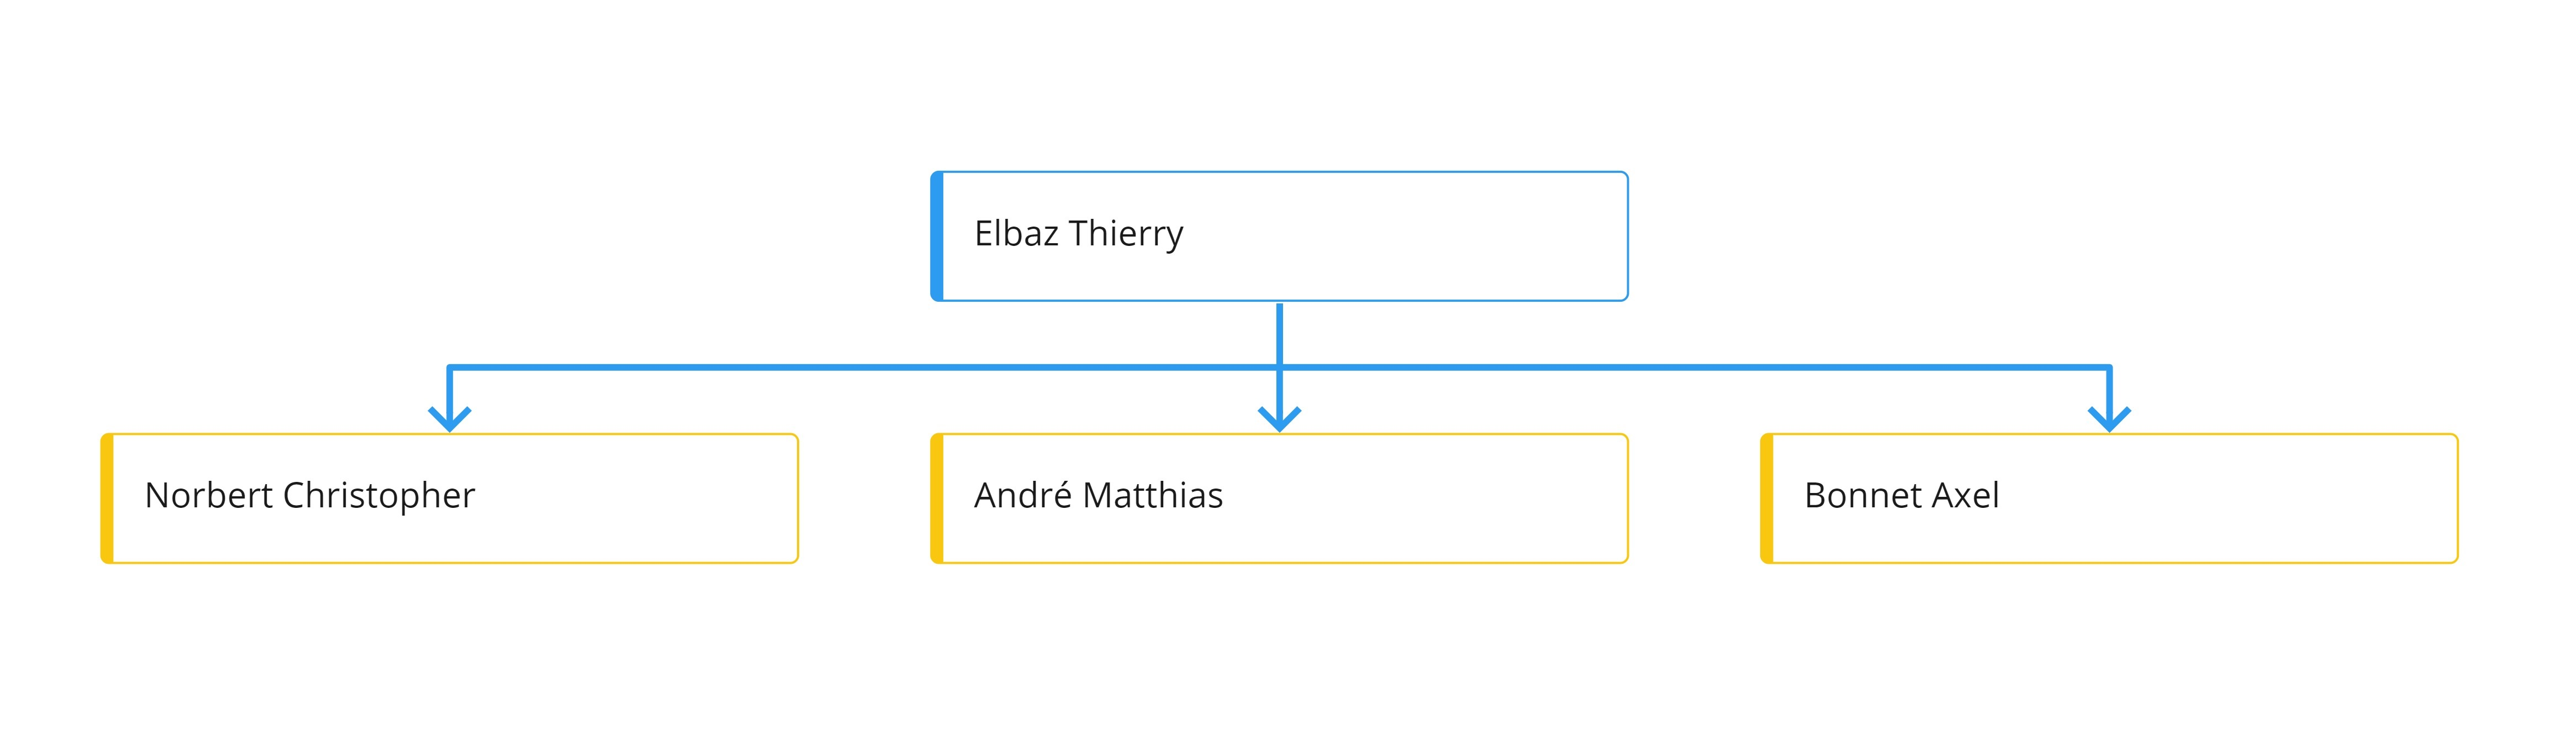
\includegraphics[width=\textwidth]{RAS chart.jpg}
    \caption{The Risk Advisory Service}
    \label{ras}
\end{figure}

\section{Work Conducted}
\subsection{Available Tools}

The company provided me with plenty of tools for me to work with, some of them were common and others were foreign and unique to this line of work. I was firstly lent a computer containing various tools in the form of software. I was also provided with a backpack, a headset, a badge, a bottle of hydro-alcoholic solution and a few reusable face masks. The software I had at my disposition were the Microsoft Office Suite, with which I was already quite familiar, and a few other software made especially for this specific work. The first one, TestComptaDemat, is used to check whether a FEC is conform in its data arrangement and field filling, performing a very superficial analysis. The second one, conformFEC, is used to analyse the FEC at a deeper level by looking into the credits and debits to generate a balance of it, as well as a summary of all the mistakes found by the software that we can highlight in our report afterwards. The third and final accounting software, FiscAudit, produces a much more complex and thorough work on the FEC. It can verify all potential mistakes, analyse the balances, the TVA and all kinds of accounts. Near the end of the internship, we were tasked with the treatment of a file which required an algorithm to do efficiently, and as such we worked with Python. I thus installed Visual Studio Code to program as I usually do with it.

\subsection{Missions}

During the course of my internship, I was given a number of missions, and all of them were of the same type, a mission we call a FEC0. As the name implies, this mission has to do with the FEC. It is a rather lighter analysis than the other more complex missions. To produce a FEC0 report, we have to treat the data provided by our clients in order to check its conformity. It must correspond to the following criterias : 
\begin{itemize}
    \item The FEC's name must contain the company's SIREN and the date of the end of the concerned fiscal year
    \item The FEC must use the appropriate encoding, separator and value formats
    \item The FEC must contain values for mandatory fields
    \item The FEC's balance must be balanced
    \item The FEC's values must be coherent
\end{itemize}
And those are only general conditions as there are a few dozens of potential anomalies inside a FEC. The mission's ultimate goal is to produce an easy to read report showing the clients the issues with his data in order for him to be able to fix them before showing his FEC to the revenue service. In order to detect such anomalies, we use the various software mentioned above. We run the FEC through the programs and analyse the outputs. Such results are often created inside multiple csv files filled with information such as the name of the error, its gravity, the lines or entries concerned. We use this data to create a visually appealing PowerPoint presentation that sums up the various anomalies for the client. See \hyperref[rapport]{an exemple here}. \\ \\
A FEC0 mission is often organised in the same way, in four different folders : 1 - Data Collection, 2 - Data Reformat, 3 - Integration and 4 - Delivrable. The first folder is used to store all the data sent by the client, such as the FEC itself, the balance sheet, the tax return, the FEC's description file and sometimes invoices. In the second folder is stored a copy of the FEC that is used to run conformFEC, whose results appear in this folder as well, and this is also where we create the 'reconciliation' sheet using the given balance and the one generated by conformFEC using the FEC. We use this sheet to point out inconsistencies and write them in the report. See \hyperref[recon]{an example here}. The third folder contains another copy of the FEC, the balance as a .txt file, and a summary of the tax return that must be filled by hand using a template and the provided files. All three files must be in a .txt format with an ANSI encoding, as this is the only type of file supported by FiscAudit, who we give the third folder as part of the mission step we call 'integration'. In the fourth folder, we store the report created by TestComptaDemat and the final PowerPoint presentation. The folder's name comes from the fact that this is the product of this mission and it is this folder that is given to the client in the end. As one can see, the mission is well organised and the folder can be used as a reminder of the various steps to follow to successfully complete a FEC0 mission.

\subsection{Tasks}

During the course of my internship, I was tasked with many missions, and underwent a bit of training, but outside of those things, I wasn't given many tasks unrelated to the FEC0 missions, aside from one very specific task. As part of its job, the Risk Advisory Service uses data sent by its clients to create reports on it after its treatment. However, sometimes the data sent is hard to treat as it is and it requires re-treatment in order for it to become usable. And this is where the task I was given comes in : to retreat the client's .xls file into a usable file, using a program. I was also to make a program of re-treatment for not only this file, but any future file of this format as well, in other words, a template. \\
The file was a balance sheet, except it had a lot of blank lines to get rid of, and was also sorted by company document references, creating a row that needed suppression yet its information had to be stored in a new column for the following rows. \\ \\
To tackle this task, I firstly decided to convert the .xls file to a .csv file, which is a really quick manual task that facilitates the program's job afterwards by a lot. Then I had to decide what programming language I was going to use, and I settled on Python, given that I knew it definitely had the ability to create an easy to understand yet efficient program that could serve as a good template, and also because I was quite familiar with it. \\
I decided to use the pandas library because of the nature of the data as a table of values, and I realised treating it as a data-frame would probably be the easier path. I then used several pandas and Python string functions such as df.notna(), df.dropna() and str.strip() to clean the document and remove the blank rows. I then struggled a bit with pandas as it was the first time I had the opportunity to use it. As such, the program I used to clean up the client's data is much more complex and less efficient than the template I came up with afterwards is. I used an infinity loop to cycle through the file's rows searching for an existing first cell that was a company name rather than a transaction ID, which meant checking whether the last character in that cell was a number or a letter. If a company name was found, its value would be stored in a temporary variable that would then be added in a specific new column at the end of each row. And the the file would be cleaned and usable for treatment. See \hyperref[py1]{this python file}. \\
Now I had a working file, and a better understanding of pandas, but I still needed to create a template out of the file that would be a lot more efficient and easier to understand. And so I did. I kept the cleaning part of the file as it was already satisfying, and as for the loop part I ended up using a simple for loop and an if condition as well as the df.loc() pandas function. This resulted in a template file being much more simple that I first thought I could create, and as such the file was left inside of BDO's servers to be used again by its employees whenever they feel a need for it. See \hyperref[py2]{the python template}.

\subsection{Training}

In order to be able to correctly execute the task I was given and fulfill the missions' objectives I had to first learn the ropes of the job. I was first instructed on how to do a FEC0 mission, and this part by part. First I learned how to collect the client's data from the company's servers. Then I learned how to use conformFEC and TestComptaDemat, and how to create a 'reconciliation' file using Excel. Then I was told how to fill in a tax return using various invoices provided by the client and a handy template. Then I learned how to use FiscAudit and how to integrate the data I treated with it. And then I learned how to use all of the above to create a neat looking PowerPoint presentation to inform the client of the various anomalies found within their financial data. \\ \\
Towards the end of my internship came the month of August, who in finance is a lot calmer than the other 11 months, most likely due to it serving as holidays for most companies and even the administration itself. At this point then we ran out of missions to complete, so my supervisor decided that we should train by ourselves on other mission types. We trained in two new mission types that were much more complex and difficult than a FEC0 mission : the VAT mission and the risk provisions mission. \\ \\
The VAT mission consists in collecting the clients' invoices from a year's months and taking several values from those documents and creating an intricate summary of them. In order to understand this mission, one must first understand how the French VAT works from a company's point of view. During a fiscal year, during various sells and purchases, a company accumulates two types of VAT : the deductible VAT and the collected VAT. A simple way to see what those two types mean it is that the collected VAT is VAT the company must pay to the State, and that deductible VAT is one that must be paid by the State to the company. Each month, depending on whether there is more collected or deductible VAT, the company must make choices that then appear on the invoices. If the collected VAT is superior to the deductible one, the company has to pay its debt to the State immediately. However, if the deductible VAT is the superior one, the company can choose whether to ask the State to be paid sometimes soon, or they can choose to keep the deductible VAT in order to compensate for the collected VAT during the following month. Such is how the VAT works for a company, and with that in mind, the summary I had to create in order to fulfill my mission had the shape of a table of values. Every VAT transaction was accounted for and filled in in chronological order using manual inputs as well as certain balance sheet imports. In the end, the obtained file was very useful in pointing out any anomaly present within the company's VAT transactions. See \hyperref[VAT]{the VAT synthesis mentioned}. \\ \\
The risk provisions mission consists in collecting monthly data obtained using FiscAudit and the client's FEC. To obtain such data, we have to extract from the complete record of transactions only certain accounts' transactions, the ones corresponding to the risk provisions. Once this is done, we need to create an Excel sheet with all of the data and we then use the Pivot Table function of Excel to calculate the sum of the targeted accounts for every month, including the RAN, the 'Report à Nouveau', which is basically every account that still contains a value by the end of the year and that is reported to the next one. And of course those accounts include also risk provisions accounts, hence why we have to use them as well. The obtained table is useful as a good summary of the risk provisions accounts, allowing the client to see if they have been distributed correctly and are coherent, as failure to be so could generate issues with the fiscal administration. See \hyperref[prov]{the risk provisions summary}.

\section{Intakes}
\subsection{Intakes within my Studies}

This internship was a very interesting experience for me. It allowed me to get a better glimpse of a professional life, and that it did a lot more than my last internship at the Departmental Council, where I had only been with a very small amount of people. This time, I discovered what an open space felt like, as it felt more like a living firm rather than an individual employee. I was also able to further increase my teamwork abilities, especially with people I met only recently. It also allowed me to look into the world of finance, which to say the least, is quite special. I am not sure whether I will ever work in this domain, given that at times it felt quite satisfying and intriguing yet at other times quite frustrating and boring. But it is a certainty that this internship was fruitful and helped me develop myself as an engineer as well. 

\subsection{The Company's Intakes}

As for the company, I have the feeling this internship was rather fruitful as well. I was able to help my colleagues with their work by doing a part of it, and it felt like after some practice I was doing some relatively good job, and I was also told so by my colleagues. I also left them with a useful re-treatment template that was mentioned in the Tasks section, which will hopefully be a good asset to the company.

\section{Conclusion}

In the end, this internship was a good experience and a great internship all in all. BDO is one of the biggest law firm there is, and the opportunity to work in such a big firm is something I feel really lucky to have obtained. I hope to find another great opportunity for my next internship, and the possibility of working again for BDO later in my life still remains.

\section{Bibliography}

\begin{itemize}
    \item Information provided by my internship supervisor and colleagues
    \item \url{https://www.bdo.fr/fr-fr/a-propos}
    \item \url{https://www.bdo.global/en-gb/about}
    \item \url{https://en.wikipedia.org/wiki/Corporate_law}
\end{itemize}

\clearpage
\section{Annexes}

\begin{figure}[h]
    \centering
    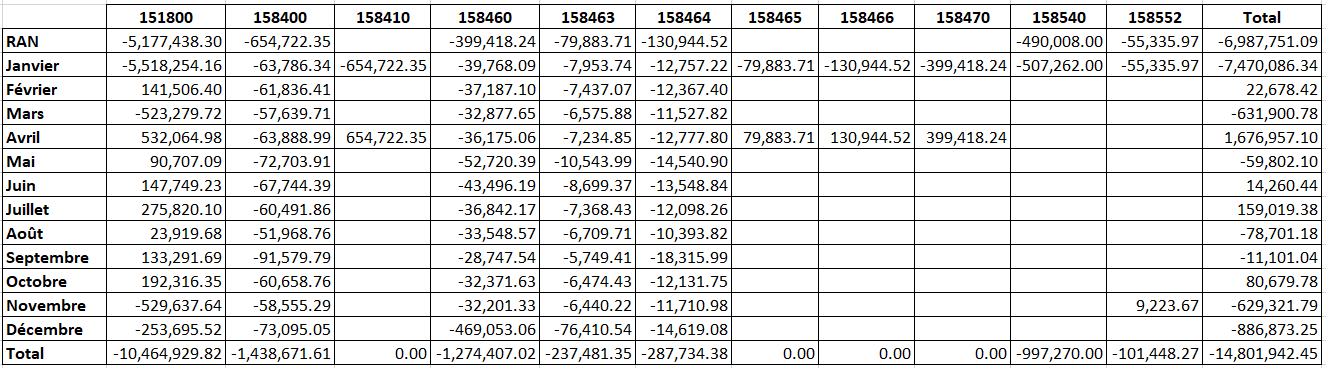
\includegraphics[width=\textwidth]{provisions.png}
    \caption{The risk provisions summary}
    \label{prov}
\end{figure}

\begin{figure}
    \centering
    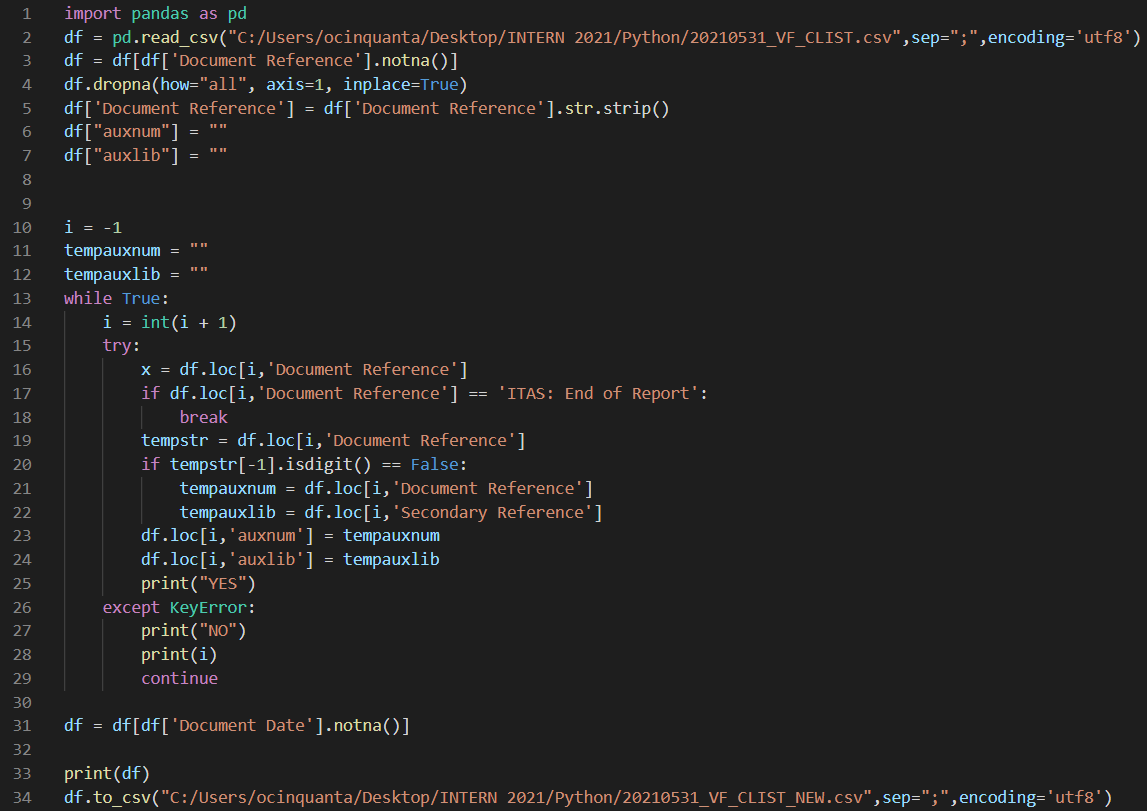
\includegraphics[width=\textwidth]{python_client.png}
    \caption{The first python file}
    \label{py1}
\end{figure}

\begin{figure}
    \centering
    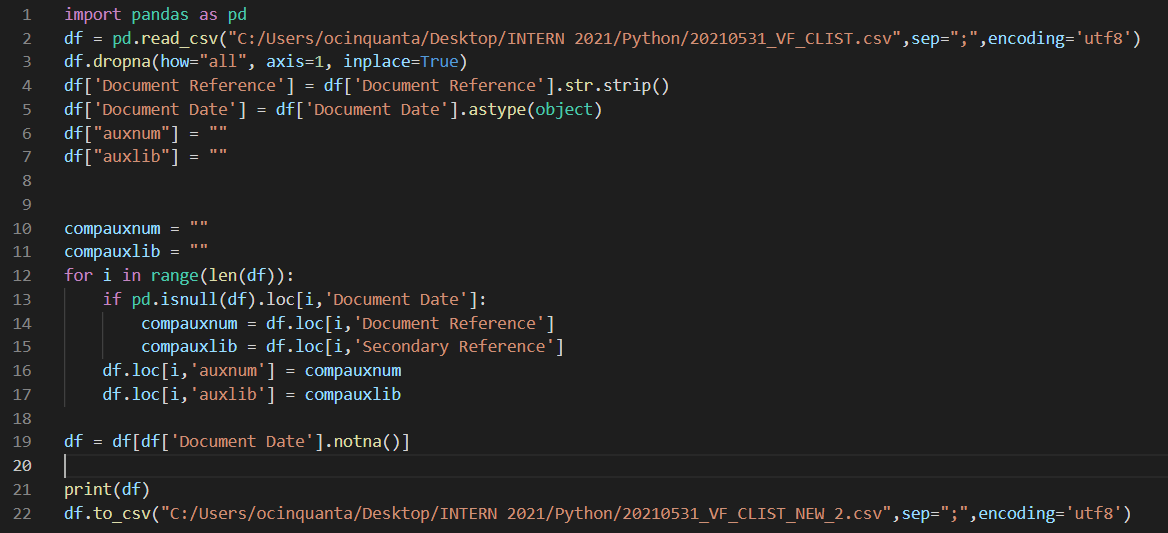
\includegraphics[width=\textwidth]{python_template.png}
    \caption{The python template}
    \label{py2}
\end{figure}

\begin{figure}
    \centering
    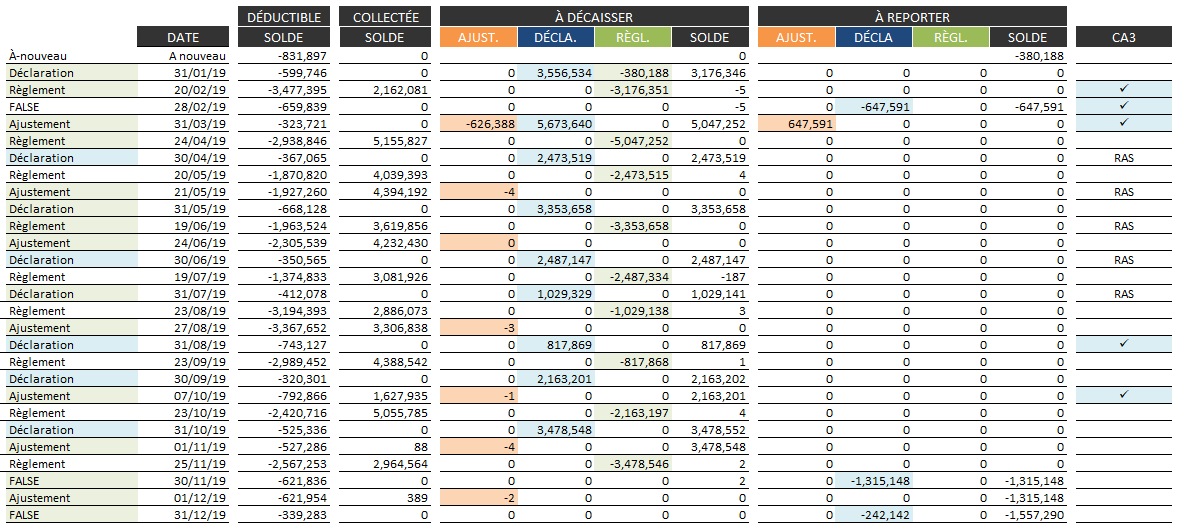
\includegraphics[width=\textwidth]{synthese_TVA.png}
    \caption{The VAT synthesis}
    \label{VAT}
\end{figure}

\begin{figure}
    \centering
    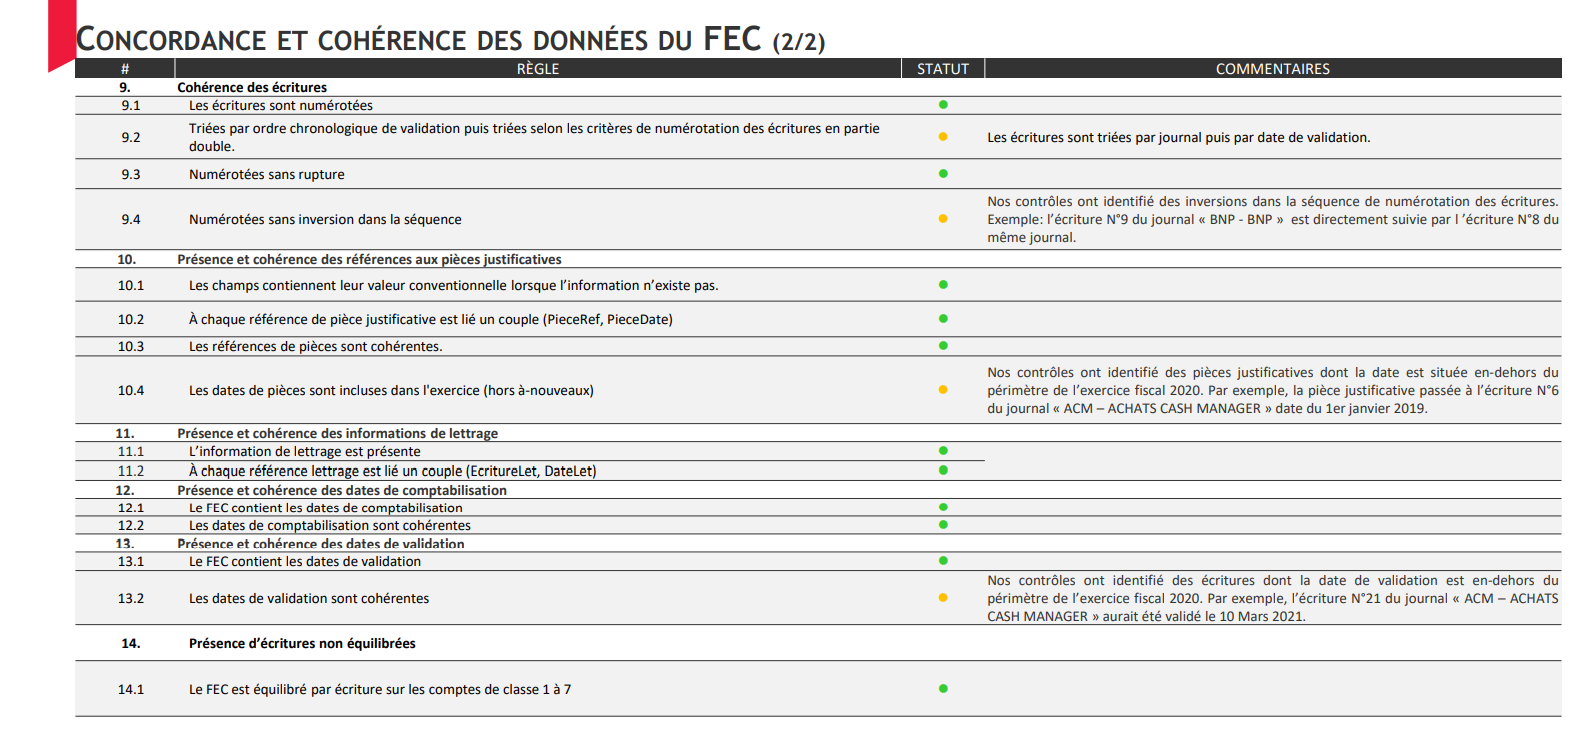
\includegraphics[width=\textwidth]{exemple_rapport.png}
    \caption{A glimpse of what the final presentation looks like}
    \label{rapport}
\end{figure}

\begin{figure}
    \centering
    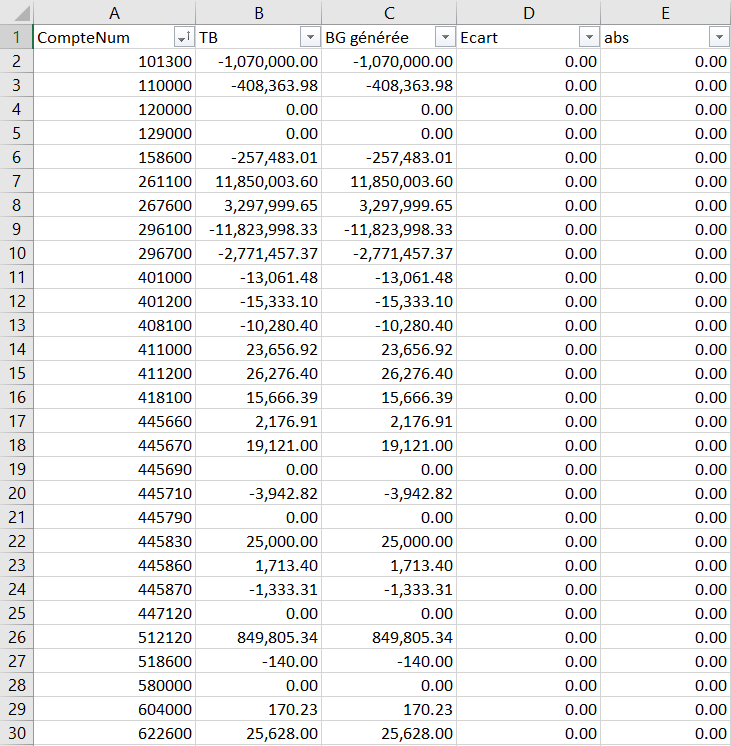
\includegraphics[width=\textwidth]{reconciliation.png}
    \caption{An example of expected 'reconciliation' file}
    \label{recon}
\end{figure}

\end{document}
